% This is samplepaper.tex, a sample chapter demonstrating the
% LLNCS macro package for Springer Computer Science proceedings;
% Version 2.20 of 2017/10/04
\documentclass[runningheads]{llncs}
\usepackage{graphicx}
\usepackage{ucs}
\usepackage[utf8]{inputenc} % upućujete LaTeX da je izvorni kod zapisan u utf8 unicode encodingu
\usepackage[T1]{fontenc} % upućujete LaTeX da koristi font family T1; ovaj redak je nužan zbog slova đ i Đ
\usepackage[boxruled,linesnumbered]{algorithm2e}
\usepackage{amssymb}
\usepackage{booktabs}
\usepackage[table,xcdraw]{xcolor}
\usepackage{placeins}
\DontPrintSemicolon
\definecolor{Gray}{gray}{0.85}
\definecolor{LightCyan}{rgb}{0.88,1,1}
\usepackage[inline]{enumitem}

\newcolumntype{g}{>{\columncolor{Gray}}c}
\begin{document}
%
\title{Automated Decision Modeling with DMN and BPMN: A Model Ensemble Approach}
%
\titlerunning{Automated Decision Modeling with DMN and BPMN}
% If the paper title is too long for the running head, you can set
% an abbreviated paper title here
%
\author{Srđan Daniel Simić\inst{1}%\orcidID{0000-1111-2222-3333}
\and
Nikola Tanković\inst{1}%\orcidID{1111-2222-3333-4444}
\and
Darko Etinger\inst{1}%\orcidID{0000-0003-4444-7202}}
}

\authorrunning{S. Daniel Simić et al.}
% First names are abbreviated in the running head.
% If there are more than two authors, 'et al.' is used.
%
\institute{Juraj Dobrila University of Pula, Faculty of Informatics, Pula, Croatia
\email{\{ssimic,ntankov,detinger\}@unipu.hr}\\
\url{https://fipu.unipu.hr/fipu/en}}
%
\maketitle              % typeset the header of the contribution
%
\begin{abstract}

Plethora of available heterogeneous transactional data and recent advancements in machine learning are the key forces that enable the development of complex algorithms that can reach human-level performance on an increasing number of tasks.

Given the non-linear structure composed of many layers of computation, these highly accurate models are usually applied in a black-box manner: without a deeper understanding of their inner mechanisms. This hinders the transparency of the decision-making process and can often incorporate hidden decision biases which are potentially present in the data.

We propose a framework for generating decision-making models conforming to Decision Model \& Notation standard based on complexity-reducing techniques. An ensemble of decision-tree classifiers in a layered architecture is proposed to control the bias-variance trade-off. We have evaluated the performance of the proposed method on several publicly available data-sets tightly related to socially sensitive decision-making.

\keywords{machine learning \and automated decision modeling \and white-box models}
\end{abstract}


\section{Introduction}

Understanding the behavior of intelligent agent algorithms is the key step in understanding what effects their outputs or decisions will have on our business processes. Generally, there is a need to reaping their benefits without accessing their harmful parts. Thus a whole new~field of science on intelligent machines as actors with~behavior and their whole surrounding ecology was recently proposed \cite{Rahwan_2019}. The ecology part of machine learning algorithms is mostly considered to be their evolution which is affected through interaction with their surroundings and exchanging new information among themselves and their business operators.

In this paper, we are interested in the decision-making automation by applying Decision Model \& Notation (DMN) \cite{DMN} coupled with well-known BPMN process automation tools \cite{BPMN}. The primary outcome of this research is a framework for modeling decision-making processes based on the previous decision outcome data by applying machine-learning techniques in a white-box manner. Understanding the model outputs, and the reasoning behind that output is the key requirement in avoiding unintentional bias.

Our contributions are the following:
\begin{enumerate*}[label=(\arabic*)]
\item
  a machine-learning ensemble method which is semantically compatible with the DMN specification, and thus human understandable,
\item
  a framework for applying this novel method on the existing decision logs - transactions of decision outcomes,
\item
  an algorithm for the automatic transformation of our proposed model into DMN artifacts.
\end{enumerate*}

The rest of the paper is organized as follows: Section \ref{sec_background} brings the definitions and motivation behind our contributions, Section \ref{sec_proposal} disseminates our contributions. Section \ref{sec_evaluation} evaluates the proposed methods on three decision-making data-sets, and Section \ref{sec_conclusion} concludes the paper with suggestions for future research.

\section{Background and Motivation}
\label{sec_background}

The implementation of algorithmic operational decisions, an important driving force for a modern organization, should not be left solely to the software engineering teams. Automated decision-making should be carefully implemented, evaluated and continuously updated with the organizational business goals.
Hence the implementation of optimal business decisions should be handled on the management level since documenting business requirements and offloading the implementation to software engineers is less efficient and error-prone due to misunderstandings. There is a level of model-driven automation present, but still it has not reach wider adoption \cite{tankovic2012rethinking}.

The transition from a classical to a digital economy has brought new challenges: the three V's of Big Data: volume, velocity, and variety make the process of decision-making a challenging one and in a need for a continuous adaptation. Machine learning models in the role of predictive analytical models are the cornerstone in seeking insight into internal and external organizational factors.

Replacing multiple decision points embedded in business processes by providing a method to derive DMN decision tables from the corresponding machine learning model was implemented in previous works \cite{Etinger_2019}. But an important challenge still remains: how to extract knowledge from increasingly complex machine learning models that try to optimize the results based on historical transactions data in which unavoidable past decision biases are deeply concealed? Failure in efficiently implementing machine learning models can lead to undesired consequences~\cite{Dressel_2018}.  The goal of Business Decision Management should be to gather insight from predictive methods, evaluate the biases and find the best trade-off in order to confidently deal with the risk of model drifts, regulatory compliance, and decision outcome performance~\cite{DMN_book}.

% \textbf{TODO}: DMN, open decisions (regulation) - human-adapted, weakness: model expressiveness, hand-crafting the models

\section{Decision framework proposal}
\label{sec_proposal}

The overall framework steps can be observed in Figure \ref{fig_workflow}. The prerequisites for the proposed framework is the implementation of the ETL process (extract-transform-load) of data from the relational database into the Decision Tool modeling environment. 

The framework is composed of three automated steps: 
\begin{enumerate*}[label=(\arabic*)]
\item Feature proposition - based on the data provided, important features are provided to the business analysts
\item DMN model proposition - a layered machine-learning model is recommended based on the chosen features, 
\item DMN table generation - automated generation of DMN tables from the proposed layered model.
\end{enumerate*}

\begin{figure}
\begin{center}
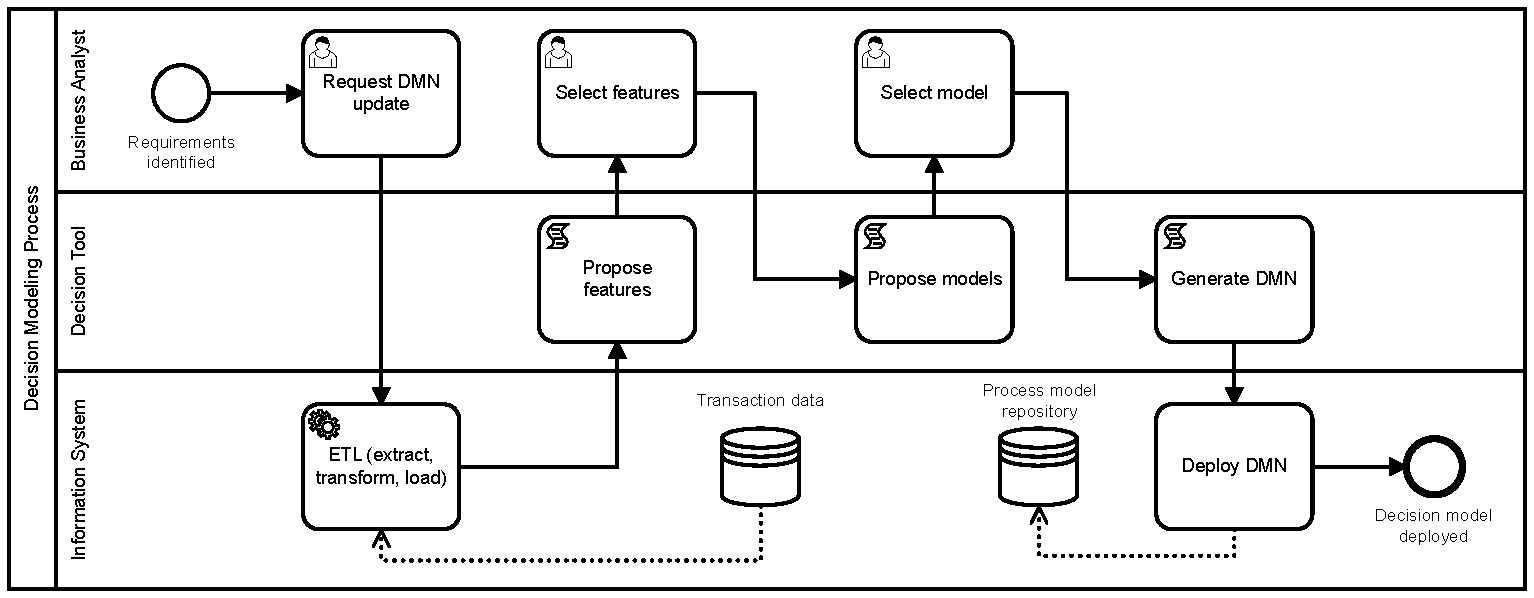
\includegraphics[width=\textwidth]{figures/usecase}
\caption{{The workflow of proposed Decision Framework}}
\label{fig_workflow}
\end{center}
\end{figure}

\subsection{Feature proposition task}

The importance of individual features $f_i \in \Phi$, is determined based on training a Gradient Boosting Machine (GBM) classifier~\cite{Ayyadevara_2018} on the data resulting from the ETL process. GBM consists of a desired number ($n$) of weak decision tree learners $wl_i, i \in [1,n]$ where feature importance corresponds to the number of splits throughout $wl_i$ decision trees, or on the average gain of the feature when it was used in the model. The score of each feature $S(f_i)$ is reported in the interval $[0, 1]$. Decision tool then reports the proposed features to the user in the descending order of importance $S(f_i)$ and automatically suggests an optimal number of features.
Optimal number of features is generating in a following way: $\hat{\Phi} = \{f_i | S(f_i) > \psi *\bar{S} \}$ where $\bar{S}$ is the mean feature importance and $\psi$ is the inclusion parameter, which we recommend to set in the range $[0.1, 0.5]$ based on the case studies we conducted. In this step special care should be given to exclude the features that should not contribute to the model according to regulations in the given domain (e.g. gender, ethnicity). 

\subsection{Model proposition task}

Based on the agreed set of features with the business analyst, the decision framework tool is able to propose an ensemble of $N_L$ decision-tree models: $\mathbb{E} = \{tm_i | i \in [1,N_L]\}$. The parameter $N_L$ is configurable and reflects the overall complexity of the desired ensemble model. The models are organized in a layered style so that model $tm_i$ suggests a decision $D(tm_i, \mathbf{x_i})$ for an input vector $\mathbf{x_i}$ only if the purity of the decision leaf $l(tm_i, \mathbf{x_i})$ is higher then the configurable threshold $\pi_i$ for that level, that is $purity(l(tm_i, \mathbf{x_i})) >= \pi_i$. Otherwise, the decision is offloaded to the next model $tm_(i+i)$. In case that $i+1 > N_L$ the final decision is left to the human operator. Such a layered composition achieves two goals:
\begin{enumerate*}[label=(\arabic*)]
    \item It a achieves a human-understandable composition of decision-tree models that can automatically be converted to DMN models,
    \item It offloads the decisions where there is lower uncertanty of the outcome to human operators.
\end{enumerate*}

\subsection{DMN model generation}

Algorithm \ref{alg_create_rows} contains the pseudo-code for generating the rules of DMN models for each decision-tree $tm_i$ on each level. Final DMN models, one per each layer are composed into the final runtime BPMN process where the final decision in the case of uncertaincy is left to human operators. Figure \ref{fig_runtime} depicts a case where $N_L = 2$.


% \begin{algorithm}[H]
%     \SetAlgoLined
%     \FuncSty{\KwSty{procedure} generateTableColumns(\ArgSty{columnNames,columnTypes})}\;
%     \Indp outputName $\leftarrow$ target class entry in columnName\;
%      inputNames $\leftarrow$ all entries in columnNames except the targeted class\;
%      \ForEach{name in inputName}{
%      createInput $\leftarrow$ create new input element of decision table\;
%      \uIf{$columnType[name]$ {\bf is} $int64$ {\bf or} $float64$ {\bf or} $int32$}{
%      createInputExpression $\leftarrow$ input expression element type double\;
%      }
%      \uElseIf{$columnType[name]$ {\bf is} $object$}{
%      createInputExpression $\leftarrow$ input expression element type string\;
%      }
%      \uElseIf{$columnType[name]$ {\bf is} $bool$}{
%      createInputExpression $\leftarrow$ input expression element type bool\;
%      }
%      \uElse{
%      createInputExpression $\leftarrow$ input expression element type date\;
%      }
%      createText $\leftarrow$ new element of input expression with value $name$
%      }
%      create output element with value in $outputName$ type string
%     \caption{Create DMN table columns}
%     \label{alg_create_columns}
% \end{algorithm}

\begin{center}
\scriptsize
\begin{minipage}{\textwidth}
\begin{algorithm}[H]
%\algsetup{linenosize=\tiny}
    \SetAlgoLined
    \FuncSty{\KwSty{procedure} generateTableRow(\ArgSty{mlDictionary, annotation, isLastTable})}\;
    \KwIn {$mlDictionary$ is dictionary containing decision tree features, thresholds and logic}
      \Indp\For{className, value in mlDictionary}{
            newRule $\leftarrow$ create new sub element of decision table\;
            \uIf{$isLastTable == True$}{
                newAnnotation $\leftarrow$ create annotation for rule with value $annotation$\;
                }
                
                \ForEach{featureName in value}{
                thresholdSignList $\leftarrow$ list of thresholds for each $featureName$\;
                    \uIf{len(thresholdSignList) == 0}{
                        ruleCell \tcp{empty in this case}\;
                    }\uElseIf{len(thresholdSignList) == 1}{
                        ruleCell $\leftarrow$ contains threshold and threshold sign\;
                        \tcp{if threshold sign is "is" or "not" threshold becomes string value}
                    }\uElse{
                        \uIf{thresholdSignList[0] is "$<=$"}{
                        \uIf{threshold[0] $>$ threshold[1]}{
                            ruleCell $\leftarrow$ create range cell 
                            }
                        }\uIf{thresholdSignList[0] is "$>$"}{
                        \uIf{threshold[0] $<$ threshold[1]}{
                            ruleCell $\leftarrow$ create range cell 
                            }
                        }    
                        \uIf{thresholdSignList[0] is "$not$" {\bf or} "$is$"}{
                                ruleCell $\leftarrow$ if  positive signs in list, write them first, negation last
                        }}}
                        
                    }
                    newOutputCell $\leftarrow$ rule sub element, contains $className$
    \caption{\small Create DMN table rows}
    \label{alg_create_rows}
\end{algorithm}
\end{minipage}
\end{center}

\begin{figure}
\begin{center}
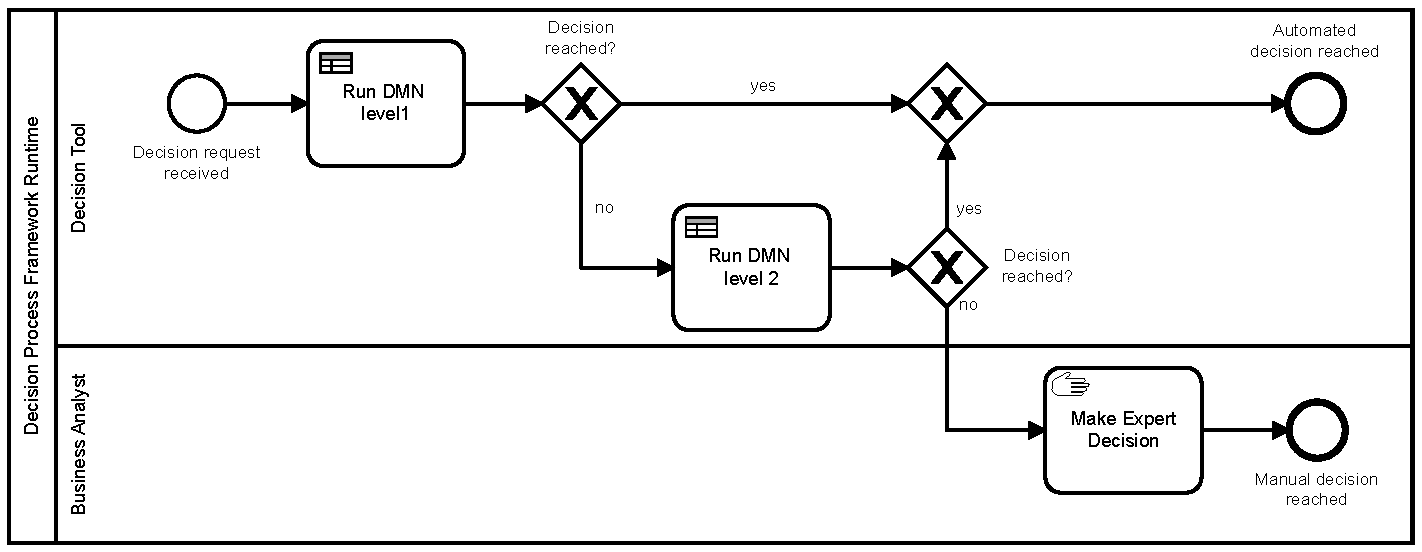
\includegraphics[width=\textwidth]{figures/runtime}
\caption{{Decision Process Framework Runtime}}
\label{fig_runtime}
\end{center}
\end{figure}
% \begin{center}
% \begin{minipage}{1.1\textwidth}
% \begin{algorithm}[H]
%     \SetAlgoLined
%     \FuncSty{\KwSty{procedure} createDecision(\ArgSty{root,previousDecision})}\;
%     \Indp xmlRoot $\leftarrow$ takes $root$ \;
%     previousPosition $\leftarrow$ takes position of previous decision table\;
%     newDecision $\leftarrow$ generates new decision element as sub element of $xmlRoot$ \;
%     newExtensionElement, newBounds $\leftarrow$ locates $newDecision$ in space \;
%     newDecisionTable $\leftarrow$ generates new decision table element as sub element of $newDecision$
    
%     \caption{Create decision table}
%     \label{alg_create_decision}
% \end{algorithm}
% \end{minipage}
% \end{center}

% \begin{center}
% \begin{minipage}{1.2\textwidth}
% \begin{algorithm}[H]
%     \SetAlgoLined
%     \FuncSty{\KwSty{procedure} createConnectionForTable(\ArgSty{firstTable, secondTable})}\;
%     \Indp startDecision, startBound $\leftarrow$ locate starting point of connection using $firstTable$ id\;
%     endDecision, endBound $\leftarrow$ locate ending point of connection using $secondTable$ id \;
%     newEdge $\leftarrow$ create edge sub element on $secondTable$\;
%     startWaypoint, endWaypoint $\leftarrow$ create waypoints sub elements of edge on the $secondTable$\;
%     newInformationRequirement$\leftarrow$ create sub elements on endDecision\;
%     newRequiredDecision $\leftarrow$ create sub element on newInformationRequirement , also needs link to $firstTable$
    
%     \caption{Create connection for tables}
%     \label{alg_create_connection}
% \end{algorithm}
% \end{minipage}
% \end{center}
% \clearpage



\newpage
\section{Evaluation}
\label{sec_evaluation}

We have evaluated our layered ensemble model on three distinct data-sets:
\begin{enumerate*}[label=(\arabic*)]
    \item Credit risk assessment dataset \footnote{\scriptsize{Available at \url{https://www.kaggle.com/uciml/german-credit}}},
    \item Medical insurance claims dataset \footnote{\scriptsize{Available at \url{https://www.kaggle.com/easonlai/sample-insurance-claim-prediction-dataset}}} and
    \item Risk of prisoner recidivism dataset
    \footnote{\scriptsize{Available at \url{https://github.com/propublica/compas-analysis}}}
\end{enumerate*}
and compared the results of the layered model against the simple decision-tree classifier and the black-box GBM model. The results are expressed through a $F1$ score \cite{Goutte:2005:PIP:2149960.2149993} and presented in Table \ref{tab_results}. Results are obtained through a 10-fold leave-one-out cross-validation technique. We can observe that from our preliminary results, our layered model with $N_L=5$ obtains more accurate results than simple decision-tree models. Such results are closer to more complex, but incomprehensible GBM models with 300 trees in ensemble. A much more comprehensive evaluation is left for future studies. It is our goal not to compare only the accuracy and the recall of the model (F1 score) but also the complexity and present the trade-offs when tuning the parameters of our layered model. Each decision generated by the GBM model in these examples is calculated from the whole set of 300 decision trees, where our approach can map a decision only to a single tree (from a specific layer). We argue that this is a significant step forward in model comprehensibility. 

% Please add the following required packages to your document preamble:
% \usepackage{booktabs}
\begin{table}[]
\footnotesize
\renewcommand{\arraystretch}{0.9}
\setlength{\tabcolsep}{0.5em} % for the horizontal padding
\begin{center}
\rowcolors{2}{gray!15}{white}
\begin{tabular}{@{}llll@{}}
\toprule
                & Decision-tree         & Layered model         & GBM                \\ \midrule
Credit-risk     & $0.700\pm0.023$       &   $0.804\pm0.028$     &   $0.830\pm0.030$  \\
Insurance claim & $0.942\pm0.021$       &   $0.952\pm0.018$     &   $0.987\pm0.011$  \\
Recidivism      & $0.644\pm0.036$       &   $0.650\pm0.019$     &   $0.654\pm0.022$  \\ \bottomrule
\end{tabular}
\end{center}
\label{tab_results}
\caption{Preliminary evaluation results based on the F1 score}
\end{table}
\FloatBarrier
\section{Conclusion}
\label{sec_conclusion}

In this paper we have presented a layered decision-tree model that is semantically compatible with the DMN specification. We have proposed a Decision-making framework and a tool for automatically building layered models and translating them into the within BPMN processes. In a brief preliminary evaluation, we have also showed that our approach reaches higher accuracy than the simple decision-tree models, support-vector machines and linear models. In the future research we plan to conduct a more thorough evaluation of our proposed methods, as well as provide an optimization framework in tuning our model parameters.

\bibliographystyle{unsrt}
\bibliographystyle{splncs04}
\bibliography{biblio}

\end{document}
